\chapter{Related Work}

% \subsection{Automating Parallelism}

It is widely accepted that parallel programming is difficult, and the
continued repetition of this claim has become something of a trite
mantra for the parallelism research community. An interesting
digression is to discuss some of the ways in which researchers have
attempted to tackle this difficult problem, and why, despite years of
research, it remains an ongoing challenge.

The most ambitious and perhaps daring field of parallelism research is
that of automatic parallelisation, where the goal is to develop
methods and systems to transform arbitrary sequential code into
parallelised code. This is a well studied subject, with the typical
approach being to perform these code transformations at the
compilation stage. In \citeauthor{Banerjee1993}'s thorough
review~\cite{Banerjee1993} on the subject, they outline the key
challenges of automatic parallelisation:
%
\begin{itemize}
	\item determining whether sequential code can be legally transformed
	for parallel execution; and
	\item identifying the transformation which will provide the highest
	performance improvement for a given piece of code.
\end{itemize}
%
Both of these challenges are extremely hard to tackle. For the former,
the difficulties lie in performing accurate analysis of code
behaviour. Obtaining accurate dynamic dependency analysis at compile
time is an unsolved problem, as is resolving pointers and points-to
analysis~\cite{Atkin-granville2013, Hind2001,Ghiya2001}.

The result of these challenges is that reliably performant, automatic
parallelisation of arbitrary programs remains a far from reached goal;
however, there are many note worthy variations on the theme which have
been able to achieve some measure of success.

One such example is speculative parallelism, which circumvents the
issue of having incomplete dependency information by speculatively
executing code regions in parallel while performing dependency tests
at runtime, with the possibility to fall back to ``safe'' sequential
execution if correctness guarantees are not
met~\cite{Prabhu2010,Trachsel2010}.  In~\cite{Jimborean2014},
\citeauthor{Jimborean2014} present a system which combines polyhedral
transformations of user code with binary algorithmic skeleton
implementations for speculative parallelisation, reporting speedups
over sequential code of up to $15.62\times$ on a 24 core processor.

Another example is PetaBricks, which is a language and compiler
enabling parallelism through ``algorithmic choice''~\cite{Ansel2009,
	Ansel2010}. With PetaBricks, users provide multiple implementations
of algorithms, optimised for different parameters or use cases. This
creates a search space of possible execution paths for a given
program. This has been combined with autotuning techniques for
enabling optimised multigrid programs~\cite{Chan2009}, with the wider
ambition that these autotuning techniques may be applied to all
algorithmic choice programs~\cite{Ansel2014}. While this helps produce
efficient parallel programs, it places a great burden on the
developer, requiring them to provide enough contrasting
implementations to make a search of the optimisation space fruitful.

Annotation-driven parallelism takes a similar approach. The user
annotates their code to provide ``hints'' to the compiler, which can
then perform parallelising transformations. A popular example of this
is OpenMP, which uses compiler pragmas to mark code sections for
parallel or vectorised execution~\cite{Dagum1998}. Previous work has
demonstrated code generators for translating OpenMP to
OpenCL~\cite{Grewe2013} and CUDA~\cite{Lee2009}. Again,
annotation-driven parallelism suffers from placing a burden on the
developer to identify the potential areas for parallelism, and lacks
the structure that algorithmic skeletons provide.

Algorithmic skeletons contrast the goals of automatic parallelisation
by removing the challenge of identifying potential parallelism from
compilers or users, instead allowing users to frame their problems in
terms of well defined patterns of computation. This places the
responsibility of providing performant, well tuned implementations for
these patterns on the skeleton author.


\section{Iterative Compilation \& Machine Learning}\label{sec:iterative-compilation}

Iterative compilation is the method of performance tuning in which a
program is compiled and profiled using multiple different
configurations of optimisations in order to find the configuration
which maximises performance. One of the the first formalised
publications of the technique appeared in \citeyear{Bodin1998} by
\citeauthor{Bodin1998}~\cite{Bodin1998}.  Iterative compilation has
since been demonstrated to be a highly effective form of empirical
performance tuning for selecting compiler optimisations.

Given the huge number of possible compiler optimisations (there are
207 flags and parameters to control optimisations in GCC v4.9), it is
often unfeasible to perform an exhaustive search of the entire
optimisation space, leading to the development of methods for reducing
the cost of evaluating configurations. These methods reduce evaluation
costs either by shrinking the dimensionality or size of the
optimisation space, or by guiding a directed search to traverse a
subset of the space.

Machine learning has been successful applied to this problem,
in~\cite{Stephenson2003}, using ``meta optimisation'' to tune compiler
heuristics through an evolutionary algorithm to automate the search of
the optimisation space. \citeauthor{Fursin2011} continued this with
Milepost GCC, the first machine learning-enabled self-tuning
compiler~\cite{Fursin2011}. A recent survey of the use of machine
learning to improve heuristics quality by \citeauthor{Burke2013}
concludes that the automatic \emph{generation} of these self-tuning
heuristics but is an ongoing research challenge that offers the
greatest generalisation benefits~\cite{Burke2013}.

% An approach to online tuning of parallel programs is presented
% in~\cite{Ansel2012} which partitions the available parallel resources
% of a device in to two partitions and then executes two different
% configurations simultaneously using each partition. The configuration
% used for one of the configuration is guaranteed to be ``safe'', and
% the performance

% % Eastep, J., Wingate, D., & Agarwal, A. (2011). Smart Data
% % Structures: An Online Machine Learning Approach to Multicore Data
% % Structures. In Proceedings of the 8th ACM International Conference
% % on Autonomic Computing (pp. 11–20). New York, NY, USA:
% % ACM. doi:10.1145/1998582.1998587
% \TODO{Online reinforcement learning for optimising data structures
%   online, \cite{Tesauro2005}}

% % Tesauro, G. (2005). Online Resource Allocation Using Decompositional
% % Reinforcement Learning. In AAAI (pp. 886–891).
% \TODO{Reinforcement learning for resource allocation~\cite{Eastep2011}}

% % W. F. Ogilvie, P. Petoumenos, Z. Wang, and H. Leather, “Intelligent
% % Heuristic Construction with Active Learning,” in 18th International
% % Workshop on Compilers for Parallel Computing, 2015.
% \TODO{Using Active Learning to speed up the learning of compiler
%   heuristics~\cite{Ogilvie2015}. Towards online autotuning, albeit
%   only with binary optimisation parameter.}

%
% SOME EXAMPLES OF ML IN THE WILD:
%

% % R. Bitirgen, E. Ipek, and J. F. Martinez, “Coordinated Management of
% % Multiple Interacting Resources in Chip Multiprocessors: A Machine
% % Learning Approach,” in 2008 41st IEEE/ACM International Symposium on
% % Microarchitecture, 2008, pp. 318–329.
% \TODO{Artificial Neural Networks for resource allocation of CMPS:
% \cite{Bitirgen2008}}

% % Z. Wang and M. F. P. O. Boyle, “Partitioning Streaming Parallelism
% % for Multi-cores: A Machine Learning Based Approach,” in Proceedings
% % of the 19th international conference on Parallel architectures and
% % compilation techniques, 2010, pp. 307–318.
% \TODO{Offline ML for partitioning streaming applications:
% \cite{Wang2010}}

In~\cite{Saclay2010,Memon2013,Fursin2014}, \citeauthor{Fursin2014}
advocate a collaborative and ``big data'' driven approach to
autotuning, arguing that the challenges facing the widespread adoption
of autotuning and machine learning methodologies can be attributed to:
a lack of common, diverse benchmarks and datasets; a lack of common
experimental methodology; problems with continuously changing hardware
and software stacks; and the difficulty to validate techniques due to
a lack of sharing in publications. They propose a system for
addressing these concerns, the Collective Mind knowledge system,
which, while in early stages of ongoing development, is intended to
provide a modular infrastructure for sharing autotuning performance
data and related artifacts across the internet. In addition to sharing
performance data, the approach taken in this thesis emphasises the
collective \emph{exploitation} of such performance data, so that data
gathered from one device may be used to inform the autotuning
decisions of another. This requires each device to maintain local
caches of shared data to remove the network overhead that would be
present from querying a single centralised data store during execution
of a hot path. The current implementation of Collective Mind uses a
NoSQL JSON format for storing performance data. The relational schema
used in this thesis offers greater scaling performance and lower
storage overhead as the amount of performance data grows.

Whereas iterative compilation requires an expensive offline training
phase to search an optimisation space, dynamic optimisers perform this
optimisation space exploration at runtime, allowing programs to
respond to dynamic features ``online''. This is a challenging task, as
a random search of an optimisation space may result in configurations
with vastly suboptimal performance. In a real world system, evaluating
many suboptimal configurations will cause a significant slowdown of
the program. Thus a requirement of dynamic optimisers is that
convergence time towards optimal parameters is minimised.

Existing dynamic optimisation research has typically taken a low level
approach to performing optimisations. Dynamo is a dynamic optimiser
which performs binary level transformations of programs using
information gathered from runtime profiling and
tracing~\cite{Bala2000}. While this provides the ability to respond to
dynamic features, it restricts the range of optimisations that can be
applied to binary transformations. These low level transformations
cannot match the performance gains that higher level parameter tuning
produces.

An interesting related tangent to iterative compilation is the
development of so-called ``superoptimisers''. In~\cite{Massalin1987},
the smallest possible program which performs a specific function is
found through a brute force enumeration of the entire instruction
set. Starting with a program of a single instruction, the
superoptimiser tests to see if any possible instruction passes a set
of conformity tests. If not, the program length is increased by a
single instruction and the process repeats. The exponential growth in
the size of the search space is far too expensive for all but the
smallest of hot paths, typically less than 13 instructions. The
optimiser is limited to register to register memory transfers, with no
support for pointers, a limitation which is addressed
in~\cite{Joshi2002}. Denali is a superoptimiser which uses constraint
satisfaction and rewrite rules to generate programs which are
\emph{provably} optimal, instead of searching for the optimal
configuration through empirical testing. Denali first translates a low
level machine code into guarded multi-assignment form, then uses a
matching algorithm to build a graph of all of a set of logical axioms
which match parts of the graph, before using boolean satisfiability to
disprove the conjecture that a program cannot be written in $n$
instructions. If the conjecture cannot be disproved, the size of $n$
is increased and the process repeats.


% \section{Performance Tuning for Heterogeneous Parallelism}

As briefly discussed in Section~\ref{sec:gpgpu}, the complex
interactions between optimisations and heterogeneous hardware makes
performance tuning for heterogeneous parallelism a difficult
task. Performant GPGPU programs require careful attention from the
developer to properly manage data layout in DRAM, caching, diverging
control flow, and thread communication. The performance of programs
depends heavily on fully utilising zero-overhead thread scheduling,
memory bandwidth, and thread grouping. \citeauthor{Ryoo2008a}
illustrate the importance of these factors by demonstrating speedups
of up to $432\times$ for matrix multiplication in CUDA by appropriate
use of tiling and loop unrolling~\cite{Ryoo2008a}. The importance of
proper exploitation of local shared memory and synchronisation costs
is explored in~\cite{Lee2010}.

In~\cite{Chen2014}, data locality optimisations are automated using a
description of the hardware and a memory-placement-agnostic
compiler. The authors demonstrate impressive speedups of up to
$2.08\times$, although at the cost of requiring accurate memory
hierarchy descriptor files for all targeted hardware. The descriptor
files must be hand generated, requiring expert knowledge of the
underlying hardware in order to properly exploit memory locality.

Data locality for nested parallel patterns is explored in~\cite{Lee}.
The authors use an automatic mapping strategy for nested parallel
skeletons on GPUs, which uses a custom intermediate representation and
a CUDA code generator, achieving $1.24\times$ speedup over hand
optimised code on 7 of 8 Rodinia benchmarks.

Reduction of the GPGPU optimisation space is demonstrated
in~\cite{Ryoo2008}, using the common subset of optimal configurations
across a set of training examples. This technique reduces the search
space by 98\%, although it does not guarantee that for a new program,
the reduced search space will include the optimal configuration.

\citeauthor{Magni2014} demonstrated that thread coarsening of OpenCL
kernels can lead to speedups in program performance between
$1.11\times$ and $1.33\times$ in~\cite{Magni2014}. The authors achieve
this using a machine learning model to predict optimal thread
coarsening factors based on the static features of kernels, and an
LLVM function pass to perform the required code transformations.

A framework for the automatic generation of OpenCL kernels from
high-level programming concepts is described in~\cite{Steuwer2015}. A
set of rewrite rules is used to transform high-level expressions to
OpenCL code, creating a space of possible implementations. This
approach is ideologically similar to that of PetaBricks, in that
optimisations are made through algorithmic choice, although in this
case the transformations are performed automatically at the compiler
level. The authors report performance on a par with that of hand
written OpenCL kernels.


% \section{Autotuning Algorithmic Skeletons}

An enumeration of the optimisation space of Intel Thread Building
Blocks in~\cite{Contreras2008} shows that runtime knowledge of the
available parallel hardware can have a significant impact on program
performance. \citeauthor{Collins2012} exploit this
in~\cite{Collins2012}, first using Principle Components Analysis to
reduce the dimensionality of the space of possible optimisation
parameters, followed by a search of parameter values to optimise
program performance by a factor of $1.6\times$ over values chosen by a
human expert. In~\cite{Collins2013}, they extend this using static
feature extraction and nearest neighbour classification to further
prune the search space, achieving an average 89\% of the oracle
performance after evaluating 45 parameters.

\citeauthor{Dastgeer2011} developed a machine learning based autotuner
for the SkePU skeleton library in~\cite{Dastgeer2011}. Training data
is used to predict the optimal execution device (i.e.\ CPU, GPU) for a
given program by predicting execution time and memory copy overhead
based on problem size. The autotuner only supports vector operations,
and there is limited cross-architecture
evaluation. In~\cite{Dastgeer2015a}, the authors extend SkePU to
improve the data consistency and transfer overhead of container types,
reporting up to a $33.4\times$ speedup over the previous
implementation.


% \section{Code Generation and Autotuning for Stencils}

Stencil codes have a variety of computationally expensive uses from
fluid dynamics to quantum mechanics. Efficient, tuned stencil kernels
are highly sought after, with early work in \citeyear{Bolz2003} by
\citeauthor{Bolz2003} demonstrating the capability of GPUs for
massively parallel stencil operations~\cite{Bolz2003}. In the
resulting years, stencil codes have received much attention from the
performance tuning research community.

\citeauthor{Ganapathi2009} demonstrated early attempts at autotuning
multicore stencil codes in~\cite{Ganapathi2009}, drawing upon the
successes of statistical machine learning techniques in the compiler
community, as discussed in
Section~\ref{sec:iterative-compilation}. They present an autotuner
which can achieve performance up to 18\% better than that of a human
expert. From a space of 10 million configurations, they evaluate the
performance of a randomly selected 1500 combinations, using Kernel
Canonical Correlation Analysis to build correlations between tunable
parameter values and measured performance targets. Performance targets
are L1 cache misses, TLB misses, cycles per thread, and power
consumption. The use of KCAA restricts the scalability of their system
as the complexity of model building grows exponentially with the
number of features. In their evaluation, the system requires two hours
of compute time to build the KCAA model for only 400 seconds of
benchmark data. They present a compelling argument for the use of
energy efficiency as an optimisation target in addition to runtime,
citing that it was the power wall that lead to the multicore
revolution in the first place. Their choice of only 2 benchmarks and 2
platforms makes the evaluation of their autotuner somewhat limited.

\citeauthor{Berkeley2009} targeted 3D stencils code performance
in~\cite{Berkeley2009}. Stencils are decomposed into core blocks,
sufficiently small to avoid last level cache capacity misses. These
are then further decomposed to thread blocks, designed to exploit
common locality threads may have within a shared cache or local
memory. Thread blocks are divided into register blocks in order to
take advantage of data level parallelism provided by the available
registers. Data allocation is optimised on NUMA systems. The
performance evaluation considers speedups of various optimisations
with and without consideration for host/device transfer overhead.

\citeauthor{Kamil2010} present an autotuning framework
in~\cite{Kamil2010} which accepts as input a Fortran 95 stencil
expression and generates tuned shared-memory parallel implementations
in Fortan, C, or CUDA. The system uses an IR to explore autotuning
transformations, enumerating a subset of the optimisation space and
recording only a single execution time for each configuration,
reporting the fastest. They demonstrate their system on 4
architectures using 3 benchmarks, with speedups of up to $22\times$
compared to serial implementations. The CUDA code generator does not
optimise for the GPU memory hierarchy, using only global memory. As
demonstrated in this thesis, improper utilisation of local memory can
hinder program performance by two orders of magnitude. There is no
directed search or cross-program learning.

In~\cite{Zhang2013a}, \citeauthor{Zhang2013a} present a code generator
and autotuner for 3D Jacobi stencil codes. Using a DSL to express
kernel functions, the code generator performs substitution from one of
two CUDA templates to create programs for execution on GPUs. GPU
programs are parameterised and tuned for block size, block dimensions,
and whether input data is stored in read only texture memory. This
creates an optimisation space of up to 200 configurations. In an
evaluation of 4 benchmarks, the authors report impressive performance
that is comparable with previous implementations of iterative Jacobi
stencils on GPUs~\cite{Holewinski2012, Phillips2010}. The dominating
parameter is shown to be block dimensions, followed by block size,
then read only memory. The DSL presented in the paper is limited to
expressing only Jacobi Stencils applications. Critically, their
autotuner requires a full enumeration of the parameter space for each
program. Since there is no indication of the compute time required to
gather this data, it gives the impression that the system would be
impractical for the needs of general purpose stencil computing. The
autotuner presented in this thesis overcomes this drawback by learning
parameter values which transfer to unseen stencils, without the need
for an expensive tuning phase for each program and architecture.
% TODO: Depending on results of cross-architecture validation, this
% last claim may not hold up.
%
% The majority of applications tested are memory bound. Does this
% transfer to computer bound?

In~\cite{Christen2011}, \citeauthor{Christen2011} presentf a DSL for
expressing stencil codes, a C code generator, and an autotuner for
exploring the optimisation space of blocking and vectorisation
strategies. The DSL supports stencil operations on arbitrarily
high-dimensional grids. The autotuner performs either an exhaustive,
multi-run Powell search, Nelder Mead, or evolutionary search to find
optimal parameter values. They evaluate their system on two CPUS and
one GPU using 6 benchmarks. A comparison of tuning results between
different GPU architectures would have been welcome, as the results
presented in this thesis show that devices have different responses to
optimisation parameters. The authors do not present a ratio of the
available performance that their system achieves, or how the
performance of optimisations vary across benchmarks or devices.

A stencil grid can be decomposed into smaller subsections so that
multiple GPUs can operate on each subsection independently. This
requires a small overlapping region where each subsection meets ---
the halo region --- to be shared between devices. For iterative
stencils, values in the halo region must be synchronised between
devices after each iteration, leading to costly communication
overheads. One possible optimisation is to deliberately increase the
size of the halo region, allowing each device to compute updated
values for the halo region, instead of requiring a synchronisation of
shared state. This reduces the communication costs between GPUs, at
the expense of introducing redundant computation. Tuning the size of
this halo region is the goal of PARTANS~\cite{Lutz2013}, an autotuning
framework for multi-GPU stencil computations. \citeauthor{Lutz2013}
explore the effect of varying the size of the halo regions using six
benchmark applications, finding that the optimal halo size depends on
the size of the grid, the number of partitions, and the connection
mechanism (i.e.\ PCI express). The authors present an autotuner which
determines problem decomposition and swapping strategy offline, and
performs an online search for the optimal halo size. The selection of
overlapping halo region size compliments the selection of workgroup
size which is the subject of this thesis. However, PARTANS uses a
custom DSL rather than the generic interface provided by SkelCL, and
PARTANS does not learn the results of tuning across programs, or
across multiple runs of the same program.

% \section{Compilers}

Using active learning to minimize the cost of iterative compilation~\cite{Ogilvie2017}.
Continuous learning of compiler heuristics~\cite{Tartara2013,Fursin2011}.

\subsection{Feature Generation for Compilers}

Machine learning has emerged as a viable means in automatically constructing heuristics for code optimization~\cite{Stephenson2005,Agakov,Wang2010,Kulkarni2012,Ding2015,Muralidharan2016}. Its great advantage is that it can adapt to changing hardware platforms as it has no a priori assumptions about their behavior. The success of machine learning based code optimization has required having a set of high-quality features that can capture the important characteristics of the target program. Given that there is an infinite number of these potential features, finding the right set of features is a non-trivial, time-consuming task.

Various forms of program features have been used in compiler-based machine learning. These include static code structures~\cite{Jiang2010} and runtime information such as system load~\cite{Wen2015} and performance counters~\cite{Dubach2009}. In compiler research, the feature sets used for predictive models are often provided without explanation and rarely is the quality of those features evaluated. More commonly, an initial large, high dimensional candidate feature space is pruned via feature selection~\cite{Stephenson2005}, or projected into a lower dimensional space~\cite{Collins2013,Dubach2007}. FEAST employs a range of existing feature selection methods to select useful candidate features~\cite{Ting2016}. Unlike these approaches, DeepTune extracts features and reduces the dimensionality of the feature space completely internally and without expert guidance.

Park \emph{et al.} present a unique graph-based approach for feature representations~\cite{Park2012}. They use a Support Vector Machine where the kernel is based on graph similarity metric. Their technique still requires hand coded features at the basic block level, but thereafter, graph similarity against each of the training programs takes the place of global features. Being a kernel method, it requires that training data graphs be shipped with the compiler, which may not scale as the size of the training data grows with the number of instances, and some training programs may be very large. Finally, their graph matching metric is expensive, requiring $O(n^3)$ to compare against each training example. By contrast, our method does not need any hand built static code features, and the deployment memory footprint is constant and prediction time is linear in the length of the program, regardless of the size of the training set.

A few methods have been proposed to automatically generate features from the compiler's intermediate representation~\cite{Namolaru2010a,Leather2014}. These approaches closely tie the implementation of the predictive model to the compiler IR, which means changes to the IR will require modifications to the model. The work of \cite{Leather2014} uses genetic programming to search for features, and required a huge grammar to be written, some 160kB in length. Although much of this can be created from templates, selecting the right range of capabilities and search space bias is non trivial and up to the expert. The work of \cite{Namolaru2010a} expresses the space of features via logic programming over relations that represent information from the IRs. It greedily searches for expressions that represent good features. However, their approach relies on expert selected relations, combinators and constraints to work. For both approaches, the search time may be significant.

Cavazos \emph{et al.\ }present a reaction-based predictive model for software-hardware co-design~\cite{Cavazos2006}. Their approach profiles the target program using several carefully selected compiler options to see how program runtime changes under these options for a given micro-architecture setting. They then use the program ``reactions'' to predict the best available application speedup. While their approach does not use static code features, developers must carefully select a few settings from a large number of candidate options for profiling, because poorly chosen options can significantly affect the quality of the model. Moreover, the program must be run several times before optimization, while our technique does not require the program to be profiled.

\section{Deep Learning for Programming Langauges}

Deep learning is a nascent branch of machine learning in which deep or multi-level graphs of processing layers are used to detect patterns in natural data~\cite{Buduma2015,LeCun2015}. It is proving especially successful for its ability to ability to process natural data in its raw form. This overcomes the traditionally laborious and time-consuming practise of engineering feature extractors to process raw data into an internal representation or feature vector. Deep learning has successfully discovered structures in high-dimensional data, and is responsible for many breakthrough achievements in machine learning, including human parity in conversational speech recognition~\cite{Xiong2016}; professional level performance in video games~\cite{Mnih2015}; and autonomous vehicle control~\cite{Lozano-Perez2012}.

In past work I used the Long Short-Term Memory (LSTM) architecture of Recurrent Neural Network (RNN)~\cite{Sundermeyer2012,Mikolov2015} to generate sequences of OpenCL code~\cite{Cummins2017a}. The LSTM network architecture comprises recurrent layers of \emph{memory cells}, each consisting of an input, output, and forget gate, and an output layer providing normalized probability values from a 1-of-K coded vocabulary~\cite{Graves,Graves2013}. Although this is the first application of deep learning for generating executable programs, RNNs have been successfully applied to a variety of other generative tasks, including image captioning~\cite{Vinyals}, colourising black and white photographs~\cite{Zhang2016}, artistic style~\cite{Gatys2015}, and image generation~\cite{Gregor2014}.

The proficiency of LSTMs for sequence modeling is demonstrated in~\cite{Sutskever2014}. \citeauthor{Sutskever2014} apply two LSTM networks to translate first a sequence into a fixed length vector, then to decode the vector into an output sequence. This architecture achieves state-of-the-art performance in machine translation. The authors find that reversing the order of the input sequences markedly improves translation performance by introducing new short term dependencies between input and output sequences. Such sequence transformations should be considered for the purpose of program generation.

The application of language modeling for generating executable programs is novel. In training on large corpuses of hand-written code, the language model learns the human biases which are present in common codes~\cite{Caliskan-islam2016}. While such human-induced basiases can prove controverial in social domains~\cite{Bolukbasi2016,Joseph2017}, this enables the generation of programs which, unlike other approaches to program generation, are representative of real workloads.

Neural networks are computationally expensive, though their implementations can be generic and parallelised. Library implementations are available in Torch~\cite{Collobert2011}, Caffe~\cite{Jia2014}, and TensorFlow~\cite{Abadi}. The increasing size and depth of computation graphs in deep learning has challenged the ability to compute results in reasonable time. Possible methods for reducing computational overhead involve fusing operations across layers in the graph using domain specific languages~\cite{Truong2016,Ashari2015a,Potter2015}; decoupling interfaces between layers using small networks to synthesise learning gradients during training~\cite{Jaderberg2016a}; and specialising hardware for computing data parallel workloads using FPGAs and ASICs~\cite{Misra2010}.


% \subsubsection{Software engineering}
Machine learning has been applied to source code to aid software engineering.  Naturalize employs techniques developed in the natural language processing domain to model coding conventions~\cite{Allamanis2014a}. JSNice leverages probabilistic graphical models to predict program properties such as identifier names for Javascript~\cite{Raychev}. \citeauthor{Zhang2015a} use deep learning to generate example code for APIs as responses to natural language queries~\cite{Zhang2015a}. \citeauthor{Allamanis2016} use attentional neural networks to generate summaries of source code~\cite{Allamanis2016}. \citeauthor{Wong2013} mines Q\&A site StackOverflow to automatically generate code comments~\cite{Wong2013}. \citeauthor{Raychev2014} use statistical models to provide contextual code completion~\cite{Raychev2014}.

There is an increasing interest in mining source code repositories at large scale~\cite{Allamanis2013a,White2015a,Bird2009}. Previous studies have involved data mining of GitHub to analyze software engineering practices~\cite{Wu2014,Guzman2014,Baishakhi2014a,Vasilescu2015}; however, no work so far has exploited mined source code for program generation.


% \subsection{Iterative compilation}

Iterative compilation is the method of performance tuning in which a program is compiled and profiled using multiple different configurations of optimisations in order to find the configuration which maximises performance. One of the the first formalised publications of the technique appeared in \citeyear{Bodin1998} by \citeauthor{Bodin1998}~\cite{Bodin1998}.  Iterative compilation has since been demonstrated to be a highly effective form of empirical performance tuning for selecting compiler optimisations.

An enumeration of the optimisation space of Intel Thread Building Blocks in~\cite{Contreras2008} shows that runtime knowledge of the available parallel hardware can have a significant impact on program performance. \citeauthor{Collins2012} exploit this in~\cite{Collins2012}, first using Principle Components Analysis to reduce the dimensionality of the optimisation space, followed by a search of parameter values to improve program performance by a factor of $1.6\times$ over values chosen by a human expert. In~\cite{Collins2013}, they extend this using static feature extraction and nearest neighbour classification to further prune the search space, achieving an average 89\% of the oracle performance after evaluating 45 parameters.

Frameworks for iterative compilation offer mechanisms for abstracting the iterative compilation process from the optimisation space. \emph{OpenTuner} presents a generic framework for optimisation space exploration~\cite{Ansel2013}. \emph{CLTune} is a generic autotuner for OpenCL kernels~\cite{Nugteren2015}. Both frameworks implement \emph{search}, however, the huge number of possible compiler optimisations makes such a search expensive to perform for every new configuration of program, architecture and dataset.

% \subsubsection{Machine learning}
Machine learning has been used to guide iterative compilation and predict optimisations for code. \citeauthor{Stephenson2003} use ``meta optimisation'' to tune compiler heuristics through an evolutionary algorithm to automate the search of the optimisation space~\cite{Stephenson2003}. \citeauthor{Fursin2011} continued this with Milepost GCC, the first machine learning-enabled self-tuning compiler~\cite{Fursin2011}. A survey of machine learning heuristics quality concludes that the automatic \emph{generation} of self-tuning heuristics is an ongoing research challenge that offers the greatest generalisation benefits~\cite{Burke2013}.

\citeauthor{Dastgeer2011} developed a machine learning based autotuner for the SkePU skeleton library in~\cite{Dastgeer2011}. Training data is used to predict the optimal execution device (i.e.\ CPU, GPU) for a given program by predicting execution time and memory copy overhead based on problem size. The autotuner only supports vector operations, and there is limited cross-architecture evaluation. In~\cite{Dastgeer2015a}, the authors extend SkePU to improve the data consistency and transfer overhead of container types, reporting up to a $33.4\times$ speedup over the previous implementation.

\citeauthor{Ogilvie2015} use active learning to reduce the cost of iterative compilation by searching for points in the optimisation space which are close to decision boundaries~\cite{Ogilvie2015}. This reduces the cost of training compared to a random search. \citeauthor{Wahib2015a} use machine learning to automate the selection of GPU kernel transformations~\cite{Wahib2015a}.

PetaBricks is a language and compiler for algorithmic choice~\cite{Ansel2009a}. Users provide multiple implementations of algorithms, optimised for different parameters or use cases. This creates a search space of possible execution paths for a given program. This has been combined with autotuning techniques for enabling optimised multigrid programs~\cite{Chan2009}, with the wider ambition that these autotuning techniques may be applied to all algorithmic choice programs~\cite{Ansel2014}. While this helps produce efficient programs, it places a great burden on the developer, requiring them to provide enough contrasting implementations to make a search of the optimisation space fruitful.

In~\cite{Saclay2010,Memon2013,Fursin2014}, \citeauthor{Fursin2014} advocate a ``big data'' driven approach to autotuning, arguing that the challenges facing widespread adoption of autotuning and machine learning methodologies can be attributed to: a lack of common, diverse benchmarks and datasets; a lack of common experimental methodology; problems with continuously changing hardware and software stacks; and the difficulty to validate techniques due to a lack of sharing in publications. They propose a system for addressing these concerns, the Collective Mind knowledge system, which provides a modular infrastructure for sharing autotuning performance data and related artifacts across the internet.


% \subsubsection{Dynamic optimisers}
Iterative compilation typically involves searching the optimisation space offline --- dynamic optimisers perform this optimisation space exploration at runtime, allowing optimisations tailored to dynamic feature values. This is a challenging task, as a random search of an optimisation space may result in many configurations with suboptimal performance. In a real world system, evaluating many suboptimal configurations will cause significant slowdowns to a program. A resulting requirement of dynamic optimisers is that convergence time towards optimal parameters is minimised.

Existing dynamic optimisation research has typically taken a low level approach to performing optimisations. Dynamo is a dynamic optimiser which performs binary level transformations of programs using information gathered from runtime profiling and tracing~\cite{Bala2000}. While this provides the ability to respond to dynamic features, it restricts the range of optimisations that can be applied to binary transformations. These low level transformations cannot match the performance gains that higher level parameter tuning produces.

% \subsubsection{Superoptimisers}
In~\cite{Massalin1987}, the smallest possible program which performs a specific function is found through an iterative enumeration of the entire instruction set. Starting with a program of a single instruction, the superoptimiser tests to see if any possible instruction passes a set of conformity tests. If not, the program length is increased by a single instruction and the process repeats. The exponential growth in the size of the search space is far too expensive for all but the smallest of hot paths, typically less than 13 instructions. The optimiser is limited to register to register memory transfers, with no support for pointers, a limitation which is addressed in~\cite{Joshi2002}. Denali is a superoptimiser which uses constraint satisfaction and rewrite rules to generate programs which are \emph{provably} optimal, instead of searching for the optimal configuration through empirical testing. Denali first translates a low level machine code into guarded multi-assignment form, then uses a matching algorithm to build a graph of all of a set of logical axioms which match parts of the graph, before using boolean satisfiability to disprove the conjecture that a program cannot be written in $n$ instructions. If the conjecture cannot be disproved, the size of $n$ is increased and the process repeats.

% \subsubsection{GPUs}
Performant GPGPU programs require careful attention from the developer to properly manage data layout in DRAM, caching, diverging control flow, and thread communication. The performance of programs depends heavily on fully utilising zero-overhead thread scheduling, memory bandwidth, and thread grouping. \citeauthor{Ryoo2008a} illustrate the importance of these factors by demonstrating speedups of up to $432\times$ for matrix multiplication in CUDA by appropriate use of tiling and loop unrolling~\cite{Ryoo2008a}. The importance of proper exploitation of local shared memory and synchronisation costs is explored in~\cite{Lee2010}.

In~\cite{Chen2014}, data locality optimisations are automated using a description of the hardware and a memory-placement-agnostic compiler. The authors demonstrate speedups of up to $2.08\times$, although at the cost of requiring accurate memory hierarchy descriptor files for all targeted hardware. The descriptor files must be hand generated, requiring expert knowledge of the underlying hardware in order to properly exploit memory locality.

Data locality for nested parallel patterns is explored in~\cite{Lee}. The authors use an automatic mapping strategy for nested parallel skeletons on GPUs, which uses a custom intermediate representation and a CUDA code generator, achieving $1.24\times$ speedup over hand optimised code on 7 of 8 Rodinia benchmarks.

Reduction of the GPGPU optimisation space is demonstrated in~\cite{Ryoo2008}, using the common subset of optimal configurations across a set of training examples. This technique reduces the search space by 98\%, although it does not guarantee that for a new program, the reduced search space will include the optimal configuration.

\citeauthor{Magni2014} demonstrated that thread coarsening of OpenCL kernels can lead to speedups in program performance between $1.11\times$ and $1.33\times$ in~\cite{Magni2014}. The authors achieve this using a machine learning model to predict optimal thread coarsening factors based on the static features of kernels, and an LLVM function pass to perform the required code transformations.

A framework for the automatic generation of OpenCL kernels from high-level programming concepts is described in~\cite{Steuwer2015}. A set of rewrite rules is used to transform high-level expressions to OpenCL code, creating a space of possible implementations. This approach is ideologically similar to that of PetaBricks, in that optimisations are made through algorithmic choice, although in this case the transformations are performed automatically at the compiler level. The authors report performance on a par with that of hand written OpenCL kernels.

% \subsubsection{Stencils}
Stencil codes have a variety of computationally expensive uses from fluid dynamics to quantum mechanics. Efficient, tuned stencil kernels are highly sought after, with early work in \citeyear{Bolz2003} by \citeauthor{Bolz2003} demonstrating the capability of GPUs for massively parallel stencil operations~\cite{Bolz2003}. In the resulting years, stencil codes have received much attention from the performance tuning research community.

\citeauthor{Ganapathi2009} demonstrated early attempts at autotuning multicore stencil codes in~\cite{Ganapathi2009}, drawing upon the successes of statistical machine learning techniques in the compiler community. They present an autotuner which can achieve performance up to 18\% better than that of a human expert. From a space of 10 million configurations, they evaluate the performance of a randomly selected 1500 combinations, using Kernel Canonical Correlation Analysis to build correlations between tunable parameter values and measured performance targets. Performance targets are L1 cache misses, TLB misses, cycles per thread, and power consumption. The use of KCAA restricts the scalability of their system as the complexity of model building grows exponentially with the number of features. In their evaluation, the system requires two hours of compute time to build the KCAA model for only 400 seconds of benchmark data. They present a compelling argument for the use of energy efficiency as an optimisation target in addition to runtime, citing that it was the power wall that lead to the multicore revolution in the first place. Their choice of only 2 benchmarks and 2 platforms makes the evaluation of their autotuner somewhat limited.

\citeauthor{Berkeley2009} targeted 3D stencils code performance in~\cite{Berkeley2009}. Stencils are decomposed into core blocks, sufficiently small to avoid last level cache capacity misses. These are then further decomposed to thread blocks, designed to exploit common locality threads may have within a shared cache or local memory. Thread blocks are divided into register blocks to take advantage of data level parallelism provided by the available registers. Data allocation is optimised on NUMA systems. The performance evaluation considers speedups of various optimisations with and without consideration for host/device transfer overhead.

\citeauthor{Kamil2010} present an autotuning framework in~\cite{Kamil2010} which accepts as input a Fortran 95 stencil expression and generates tuned shared-memory parallel implementations in Fortan, C, or CUDA. The system uses an IR to explore autotuning transformations, enumerating a subset of the optimisation space and recording only a single execution time for each configuration, reporting the fastest. They demonstrate their system on 4 architectures using 3 benchmarks, with speedups of up to $22\times$ compared to serial implementations. The CUDA code generator does not optimise for the GPU memory hierarchy, using only global memory. As demonstrated in this thesis, improper utilisation of local memory can hinder program performance by two orders of magnitude. There is no directed search or cross-program learning.

In~\cite{Zhang2013a}, \citeauthor{Zhang2013a} present a code generator and autotuner for 3D Jacobi stencil codes. Using a DSL to express kernel functions, the code generator performs substitution from one of two CUDA templates to create programs for execution on GPUs. GPU programs are parameterised and tuned for block size, block dimensions, and whether input data is stored in read only texture memory. This creates an optimisation space of up to 200 configurations. In an evaluation of 4 benchmarks, the authors report performance that is comparable with previous implementations of iterative Jacobi stencils on GPUs~\cite{Holewinski2012, Phillips2010}. The dominating parameter is shown to be block dimensions, followed by block size, then read only memory. The DSL presented in the paper is limited to expressing only Jacobi Stencils applications. Their autotuner requires a full enumeration of the parameter space for each program, which may be impractical for the needs of general purpose stencil computing. Previous work (Appendix~\ref{app:adapt}) overcomes this drawback by learning parameter values which transfer to unseen stencils, without the need for an expensive tuning phase for each program and architecture.

In~\cite{Christen2011}, \citeauthor{Christen2011} presents a DSL for expressing stencil codes, a C code generator, and an autotuner for exploring the optimisation space of blocking and vectorisation strategies. The DSL supports stencil operations on arbitrarily high-dimensional grids. The autotuner performs either an exhaustive, multi-run Powell search, Nelder Mead, or evolutionary search to find optimal parameter values. They evaluate their system on two CPUS and one GPU using 6 benchmarks. The authors do not present a ratio of the available performance that their system achieves, or how the performance of optimisations vary across benchmarks or devices.

A stencil grid can be decomposed into smaller subsections so that multiple GPUs can operate on each subsection independently. This requires a small overlapping region where each subsection meets --- the halo region --- to be shared between devices. For iterative stencils, values in the halo region must be synchronised between devices after each iteration, leading to costly communication overheads. One possible optimisation is to deliberately increase the size of the halo region, allowing each device to compute updated values for the halo region, instead of requiring a synchronisation of shared state. This reduces the communication costs between GPUs, at the expense of introducing redundant computation. Tuning the size of this halo region is the goal of PARTANS~\cite{Lutz2013}, an autotuning framework for multi-GPU stencil computations. \citeauthor{Lutz2013} explore the effect of varying the size of the halo regions using six benchmark applications, finding that the optimal halo size depends on the size of the grid, the number of partitions, and the connection mechanism (i.e.\ PCI express). The authors present an autotuner which determines problem decomposition and swapping strategy offline, and performs an online search for the optimal halo size. The selection of overlapping halo region size compliments the selection of workgroup size which is the subject of previous work (Appendix~\ref{app:adapt}).

In applications of machine learning for iterative compilation, a limiting factor of the effectiveness of learned models is the number of benchamrks used. The development of automatic program generation alleviates this problem by allowing an unbounded number of programs to enumerate the feature space at an increasingly granular scale.


% \subsection{Learning Representations}

Recently, deep neural networks~\cite{LeCun2015} have been shown to be a powerful tool for feature engineering in various tasks including image recognition~\cite{Krizhevsky2012,He2016} and audio processing~\cite{Lee2009b}. In the field of compiler optimization, no work so far has applied deep neural networks for program feature generation and selection. Our work is the first to do so.

% \subsection{Generative Modeling}

Generative models for video~\cite{Srivastava2015}.

%% Jozefowicz, R., Vinyals, O., Schuster, M., Shazeer, N., & Wu, Y. (2016). Exploring the Limits of Language Modeling. arXiv:1602.02410. Retrieved from http://arxiv.org/abs/1602.02410%5Cnhttp://www.arxiv.org/pdf/1602.02410.pdf
Limits of language modeling~\cite{Jozefowicz2016a}.

%% Sutskever, I., Vinyals, O., & Le, Q. V. (2014). Sequence to Sequence Learning with Neural Networks. In NIPS.
Sequence to sequence learning, NIPS paper~\cite{Sutskever2014}.

%% Wang, H., Raj, B., & Xing, E. P. (2017). On the Origin of Deep Learning, 1–81. Retrieved from http://arxiv.org/abs/1702.07800
Deep Learning is an emerging branch of machine learning, offering breakthrough domains in a number of domains~\cite{Wang2017}.

Automatic inference from raw inputs in other fields. Review of representation learning~\cite{Bengio2013}. Object detection, image classification, text classification~\cite{Conneau2016}, and even to the optimizations themselves~\cite{Andrychowicz2016a}. We are the first to apply this approach to compilers.

End to end training of robotic control policies~\cite{Levine2016}.



% \subsection{Transfer Learning}

%% Razavian, A. S., Azizpour, H., Sullivan, J., & Carlsson, S. (2014). CNN Features off-the-shelf: an Astounding Baseline for Recognition. In CVPRW. https://doi.org/10.1109/CVPRW.2014.131
Exploring relevance of inferred features in model hidden layers~\cite{Yosinski2014}. Transfer learning is common in other domains, e.g. vision~\cite{Razavian2014,Oquab2014}. Often using the hidden layers as fixed feature extractors (by using the output of one sub-model as input to a new model), rather than using the same model structure and transferring weights (as we did).


\subsection{Mining Source Code}

There is an increasing interest in mining source code repositories at large scale~\cite{Allamanis2013a,White2015a,Bird2009}. Previous studies have involved data mining of GitHub to analyze software engineering practices~\cite{Wu2014,Guzman2014,Baishakhi2014a,Vasilescu2015}, for example code generation~\cite{Zhang2015a}, code summarization~\cite{Allamanis2016}, comment generation~\cite{Wong2013}, and code completion~\cite{Raychev2014}. However, no work so far has exploited mined source code for benchmark generation. This work is the first to do so.

In recent years, machine learning techniques have been employed to model and learn from program source code on various tasks. These include mining coding conventions~\cite{Allamanis2014a} and idioms~\cite{Allamanis2014}, API example code~\cite{Zhang2015a} and pseudo-code generation~\cite{Oda2015}, and benchmark generation~\cite{Cummins2017a}. Our work is the first attempt to extend the already challenging task of modeling distributions over source code to learning distributions over source code with respect to code optimizations.

In a recent work~\cite{Bunel2017a}, Bunel \emph{et al.} formulate code super-optimization as a stochastic search problem to learn the distribution of different code transformations and expected performance improvement. As acknowledged by the authors, their approach can be improved by having temporal information of the code structures.


\section{Program Generation}

\emph{GENESIS}~\cite{Chiu2015} is a language for generating synthetic training programs. The essence of the approach is to construct a probabilistic grammar with embedded semantic actions that defines a language of possible programs. New programs may be created by sampling the grammar and, through setting probabilities on the grammar productions, the sampling is biased towards producing programs from one part of the space or another. This technique is potentially completely general, since a grammar can theoretically be constructed to match any desired program domain. However, despite being theoretically possible, it is not easy to construct grammars which are both suitably general and also produce programs that are in any way similar to human written programs. It has been shown to be successful over a highly restricted space of stencil benchmarks with little control flow or program variability~\cite{Garvey2015b,Falch2015} (Appendix~\ref{app:adapt}). But, it is not clear how much effort it will take, or even if it is possible for human experts to define grammars capable of producing human like programs in more complex domains. By contrast, learning from a corpus provides \emph{general-purpose} program generation over unknown domains, in which the statistical distribution of generated programs is automatically inferred from real world code.

Random program generation is an effective method for software testing. Grammar-based \emph{fuzz testers} have been developed for C~\cite{Yang2012} and OpenCL~\cite{Lidbury2015a}. Programs generated by grammar-based approaches are often  unlike real handwritten code, and are typically very large. As such, once a bug has been identified, test case reduction~\cite{Regehr2012a} is required to minimise the size of the program and isolate the code of interest. A mutation-based approach for differential testing the Java Virtual Machine is demonstrated in~\cite{Chena}.

Goal-directed program generators have been used for a variety of domains, including generating linear transforms~\cite{Voronenko2009}, MapReduce programs~\cite{Smith}, and data structure implementations~\cite{Loncaric2016}.

\subsection{Training with Synthetic Benchmarks}

The use of synthetic benchmarks for providing empirical performance
evaluations dates back to as early as 1974~\cite{Curnow1976}. The
\emph{automatic generation} of such synthetic benchmarks is a more
recent innovation, serving the purpose initially of stress-testing
increasingly complex software systems for behaviour validation and
automatic bug detection~\cite{Verplaetse2000,Godefroid2008}. A range
of techniques have been developed for these purposes, ranging from
applying random mutations to a known dataset to generate test stimuli,
to so-called ``whitebox fuzz testing'' which analyses program traces
to explore the space of a program's control flow. Csmith is one such
tool which generates randomised C source programs for the purpose of
automatically detecting compiler bugs~\cite{Yang2012}.

A method for the automatic generation of synthetic benchmarks for the
purpose of \emph{performance} tuning is presented
in~\cite{Chiu2015}. \citeauthor{Chiu2015} use template substitution
over a user-defined range of values to generate training programs with
a statistically controlled range of features. A Perl preprocessor
generates output source codes from an input description using a custom
input language Genesis. Genesis is more flexible than the system
presented in this thesis, supporting substitution of arbitrary
sources. The authors describe an application of their tool for
generating OpenCL stencil kernels, but do not report any performance
results.

\emph{GENESIS}~\cite{Chiu2015} is a language for generating synthetic training programs. Users annotate template programs with statistical distributions over features, which are instantiated to generate statistically controlled permutations of templates. Template based approaches provide domain-specific solutions for a constrained feature and program space, for example, generating permutations of Stencil codes~\cite{Garvey2015b,Cummins2015a}. Our approach provides \emph{general-purpose} program generation over unknown domains, in which the statistical distribution of generated programs is automatically inferred from real world code.

Random program generation is an effective method for software testing. Grammar-based \emph{fuzz testers} have been developed for C~\cite{Yang2012} and OpenCL~\cite{Lidbury2015a}. A mutation-based approach for the Java Virtual Machine is demonstrated in~\cite{Chena}. Goal-directed program generators have been used for a variety of domains, including generating linear transforms~\cite{Voronenko2009}, MapReduce programs~\cite{Smith}, and data structure implementations~\cite{Loncaric2016}. Program synthesis from input/output examples is used for simple algorithms in~\cite{Zaremba2015a}, string manipulation in~\cite{Gulwani2011}, and geometry constructions in~\cite{Gulwani2012}.

Machine learning has been applied to source code to aid software engineering. Naturalize employs techniques developed in the natural language processing domain to model coding conventions~\cite{Allamanis2014a}. JSNice leverages probabilistic graphical models to predict program properties such as identifier names for Javascript~\cite{Raychev}.


%\subsection{Parallelism}
%
%Programming languages have taken a variety of approaches in adopting parallelism. In C, a threading model was retrofitted using the \textit{POSIX pthreads} standard~\cite{Sura2005}. \citeauthor{Boehm2005} contends this approach in~\cite{Boehm2005}, describing issues in which a compiler developed independently of threading issues cannot be guaranteed to produce correct code. These issues were circumvented in C++11 by the introduction of a concurrency model~\cite{Boehm2008}, based off the success of the Java memory model~\cite{Bash2015a}. C++ and Java are two of the most popular imperative programming languages, and in both cases, the languages specify memory models which guarantee sequential consistency across threads, subject to some restrictions. A dialect of the Java programming language, Titanium, extends the Java feature set, adding multidimensional arrays, immutable classes, and a PGAS programming model~\cite{Yelick1998}. In contrast, Deterministic Parallel Java adds a type and effect system to in order to provide a provably sound language core~\cite{Bocchino2009}.
%
%
%%
%%% \subsubsection{Limits of static analysis}
%%Sequential consistency in shared-memory parallel programming~\cite{Krishnamurthy1995,Shasha1988,Sura2005}. Sequential consistency and caches~\cite{Goodman}.
%%
%%Sequential consistency for Java incurs a 10\% slowdown~\cite{Sura2005}.
%%
%
%%
%%Parallelism in the modern functional languages: Haskell, Clojure and Erlang~\cite{Pierro2012}.
%%
%%Scala actors~\cite{Haller2009a}, and~\cite{Haller2012}.
%%
%%
%%\subsubsection{Library level parallelism} Optimising MapReduce for multi-core processors~\cite{Kaashoek2010}.
%%TODO: OpenMP, MPI
%
%
%\subsubsection{Automatic parallelisation} The goal of automatic parallelisation is to transform arbitrary sequential code into parallelised code. This is a well studied subject, with the typical approach being to perform these code transformations at the compilation stage. In \citeauthor{Banerjee1993}'s thorough review~\cite{Banerjee1993} of the subject, they outline the key challenges of automatic parallelisation: determining whether sequential code can be legally transformed for parallel execution; and identifying the transformation which will provide the highest performance improvement for a given piece of code. Both challenges are hard to tackle. For the former, the difficulties lie in performing accurate analysis of code behaviour. Obtaining accurate dynamic dependency analysis at compile time is an unsolved problem, as is resolving pointers and points-to analysis~\cite{Atkin-granville2013, Hind2001,Ghiya2001}.
%
%The result of these challenges is that reliably performant, automatic parallelisation of arbitrary programs remains a far reaching goal; however, there are noteworthy variations on which have been able to achieve some measure of success. One such example is speculative parallelism, which circumvents the issue of having incomplete dependency information by speculatively executing code regions in parallel while performing dependency tests at runtime, with the possibility to fall back to ``safe'' sequential execution if correctness guarantees are not met~\cite{Prabhu2010,Trachsel2010}.  In~\cite{Jimborean2014}, \citeauthor{Jimborean2014} present a system which combines polyhedral transformations of user code with binary algorithmic skeleton implementations for speculative parallelisation, reporting speedups over sequential code of up to $15.62\times$ on a 24 core processor.
%
%Annotation-driven parallelism takes a similar approach. The user annotates their code to provide ``hints'' to the compiler, which can then perform parallelising transformations. A popular example of this is OpenMP, which uses compiler pragmas to mark code sections for parallel or vectorised execution~\cite{Dagum1998}. Previous work has demonstrated code generators for translating OpenMP to OpenCL~\cite{Grewe2013} and CUDA~\cite{Lee2009}. Again, annotation-driven parallelism suffers from placing a burden on the developer to identify the potential areas for parallelism, and lacks the structure that algorithmic skeletons provide.


%
%
%\subsubsection{Debugging}
%General purpose, platform-specific debuggers: Intel Debugger for Linux~\cite{Blair-chappell}.
%
%
%% \subsubsection{Debugging Parallel Frameworks and Libraries}
%
%Allinea DDT~\cite{K2010}, a scalable parallel debugger.
%
%TotalView~\cite{Cownie2000}, an OpenMP debugger.
%
%Jumbune~\cite{ImpetusTechnologies}, an open source debugger for Hadoop.
%
%The parallel pipeline library FlumeJava~\cite{Chambers2010} provides debugging support through regular tools using a sequential execution mode,r and routing of exceptions and output from remote workers back to a central host.
%
%
%% \subsubsection{Debugging GPGPU programs}
%
%CUDA-GDB~\cite{NVIDIA2016}, Intel OpenCL Debugger for Linux
%OS~\cite{IntelCorporation2016}.
%
%Oclgrind~\cite{Price2015}.
%
%GPUverify~\cite{Betts2012}.
%
%
%% \subsubsection{Debugging Algorithmic Skeletons}
%SkIE~\cite{Bacci1999} is based on a coordination language, but provides advanced features such as debugging tools, performance analysis, visualization, and graphical user interface. Instead of directly using the coordination language, programmers interact with a graphical tool, where parallel modules based on skeletons can be composed
%
%SKiPPER~\cite{Serot1999} supports sequential execution for debugging.
%
%
%\subsubsection{Profiling}
%Profiling sequential programs~\cite{Ball1994}.
%
%% \subsubsection{Profiling parallel programs}
%Profiling parallel programs using KOJAK~\cite{Mohr2003}.
%
%


%\subsection{Performance Benchmarking}
%
%Rodinia~\cite{Che2009,Che2010},
%NPB (SNU~\cite{Seo2011}),
%Parboil~\cite{Stratton2012},
%PolyBench~\cite{Grauer-Gray2012},
%SHOC~\cite{Danalis2010}.
%
%Evaluating GPGPU benchmarks~\cite{Ryoo2015}.
%
%Benchmarking parallel computing systems~\cite{Belli2015}.
%
%\subsubsection{Methodology} Use geometric mean for speedups~\cite{Fleming1986}. Statistical rigour\cite{Georges2007}. Execution times and variance~\cite{Box}.
%
%\subsection{Self-Tuning Software}
%



% TODO(cec): CGO'17 related wrok section:


Our work lies at the intersections of a number of areas: program generation, benchmark characterization, and language modeling and learning from source code. There is no existing work which is similar to ours, in respect to learning from large corpuses of source code for benchmark generation.

\emph{GENESIS}~\cite{Chiu2015} is a language for generating synthetic training programs. Users annotate template programs with statistical distributions over features, which are instantiated to generate statistically controlled permutations of templates. Template based approaches provide domain-specific solutions for a constrained feature and program space, for example, generating permutations of Stencil codes~\cite{Garvey2015b,Cummins2015a}. Our approach provides \emph{general-purpose} program generation over unknown domains, in which the statistical distribution of generated programs is automatically inferred from real world code.

Random program generation is an effective method for software testing. Grammar-based \emph{fuzz testers} have been developed for C~\cite{Yang2012} and OpenCL~\cite{Lidbury2015a}. A mutation-based approach for the Java Virtual Machine is demonstrated in~\cite{Chena}. Goal-directed program generators have been used for a variety of domains, including generating linear transforms~\cite{Voronenko2009}, MapReduce programs~\cite{Smith}, and data structure implementations~\cite{Loncaric2016}. Program synthesis from input/output examples is used for simple algorithms in~\cite{Zaremba2015a}, string manipulation in~\cite{Gulwani2011}, and geometry constructions in~\cite{Gulwani2012}.

Machine learning has been applied to source code to aid software engineering. Naturalize employs techniques developed in the natural language processing domain to model coding conventions~\cite{Allamanis2014a}. JSNice leverages probabilistic graphical models to predict program properties such as identifier names for Javascript~\cite{Raychev}.

There is an increasing interest in mining source code repositories at large scale~\cite{Allamanis2013a,White2015a,Bird2009}. Previous studies have involved data mining of GitHub to analyze software engineering practices~\cite{Wu2014,Guzman2014,Baishakhi2014a,Vasilescu2015}, for example code generation~\cite{Zhang2015a}, code summarization~\cite{Allamanis2016}, comment generation~\cite{Wong2013}, and code completion~\cite{Raychev2014}. However, no work so far has exploited mined source code for benchmark generation. This work is the first to do so.


% TODO(cec):  ISSTA'18 related work section:

The random generation of test cases is a well established approach to the
compiler validation problem. Prior approaches are surveyed
in~\cite{Kossatchev2005,Boujarwah1997} and empirically contrasted
in~\cite{Chen2014a}. The main question of interest is in how to efficiently
generate codes which trigger bugs. There are two main approaches: \emph{program
	generation}, where inputs are synthesized from scratch; and \emph{program
	mutation}, where existing codes are modified so as to identify anomalous
behavior.

\begin{figure}
	\centering %
	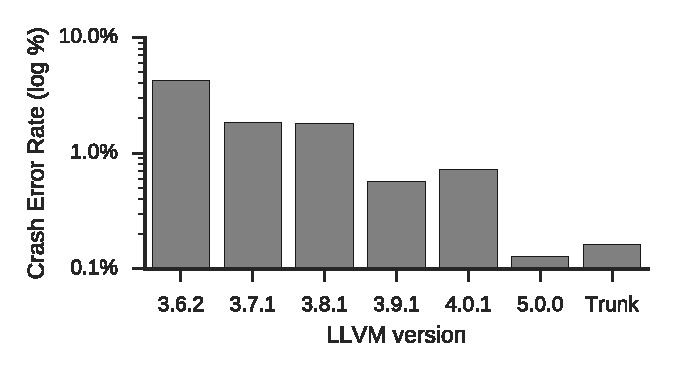
\includegraphics[width=.85\columnwidth]{img/clang-crashes}%
	\vspace{-2em}
	\caption{%
		Crash rate of the Clang front-end of every LLVM release in the past 24
		months compiling 75k DeepSmith kernels.%
	}%
	\vspace{-1em}
	\label{fig:clangs}
	%
\end{figure}
\begin{table}
	\footnotesize %
	\centering %
	\caption{%
		The number of DeepSmith programs which trigger distinct Clang front-end
		assertions, and the number of programs which trigger unreachables.%
	}
	\vspace{-1.5em}
	\begin{tabular}{r|ccccccc}
  \toprule
  {} & 3.6.2 & 3.7.1 & 3.8.1 & 3.9.1 & 4.0.1 & 5.0.0 & Trunk \\
  \midrule
  Assertion 1 & 2962 & 1327 & 1332 & 414 & 523 & 83 & 97 \\
  Assertion 2 & & 1 & 1 & & & &       \\
  Assertion 3 & & & & & & & 1 \\
  Assertion 4 & & & & & & & 2 \\
  Assertion 5 & 147 & & & & & &       \\
  Assertion 6 & 1 & & & & & &       \\
  Assertion 7 & & & & 1 & 1 & &       \\
  Unreachable & 86 & 42 & 14 & 14 & 18 & 13 & 21 \\
  \bottomrule
\end{tabular}

	\label{tab:clangs}
\end{table}

\paragraph{Program Generation}

In the foundational work on differential testing for compilers, McKeeman
\emph{et al.\ }present generators capable of enumerating programs of a range of
qualities, from random ASCII sequences to C model conforming
programs~\cite{McKeeman1998}. Subsequent works have presented increasingly
complex generators which improve in some metric of interest, generally
expressiveness or probability of correctness. CSmith~\cite{Yang2011} is a widely
known and effective generator which enumerates programs by pairing infrequently
combined language features. In doing so, it produces correct programs with
clearly defined behavior but very unlikely functionality, increasing the chances
of triggering a bug. Achieving this required extensive engineering work, most of
it not portable across languages, and ignoring some language features.
Subsequent generators influenced by CSmith, like Orange3~\cite{Nagai2013}, focus
on features and bug types beyond the scope of CSmith, arithmetic bugs in the
case of Orange3. Glade~\cite{Bastani2017} derives a grammar from a corpus of
example programs. The derived grammar is enumerated to produce new programs,
though unlike our approach, no distribution is learned over the grammar; program
enumeration is uniformly random.

\paragraph{Program Mutation}

Equivalence Modulo Inputs (EMI) testing~\cite{Le2013a,Sun2016a} follows a
different approach to test case generation. Starting with existing code, it
inserts or deletes statements that will not be executed, so functionality should
remain the same. If it is affected, it is due to a compiler bug. While a
powerful technique able to find hard to detect bugs, it relies on having a very
large number of programs to mutate. As such, it still requires an external code
generator. Similarly to CSmith, EMI favors very long test programs.
LangFuzz~\cite{Holler2012} also uses mutation but does this by inserting code
segments which have previously exposed bugs. This increases the chances of
discovering vulnerabilities in scripting language engines. Skeletal program
enumeration~\cite{Zhang2017a} again works by transforming existing code. It
identifies algorithmic patterns in short pieces of code and enumerates all the
possible permutations of variable usage. Compared to all these, our fuzzing
approach is low cost, easy to develop, portable, capable of detecting a wide
range of errors, and focusing by design on bugs that are more likely to be
encountered in a production scenario.

\paragraph{Machine Learning}

There is an increasing interest in applying machine learning to software
testing. Most similar to our work is Learn\&fuzz~\cite{Godefroid2017}, in which
an LSTM network is trained over a corpus of PDF files to generate test inputs
for the Microsoft Edge renderer, yielding one bug. Unlike compiler testing, PDF
test cases require no inputs and no pre-processing of the training corpus.
Skyfire~\cite{Wang2017c} learns a probabilistic context-sensitive grammar over a
corpus of programs to generate input seeds for mutation testing. The generated
seeds are shown to improve the code coverage of AFL~\cite{Zalewski} when fuzzing
XSLT and XML engines, though the seeds are not directly used as test cases.
Machine learning has also been applied to other areas such as improving bug
finding static analyzers~\cite{Heo2017,Koc2017}, repairing
programs~\cite{Koukoutos2017a,White}, prioritizing test
programs~\cite{Chen2017}, identifying buffer overruns~\cite{Choi2016}, and
processing bug reports~\cite{Lam2016,Huo2016}. To the best of our knowledge, no
work so far has succeeded in finding compiler bugs by exploiting the learned
syntax of mined source code for test case generation. Ours is the first to do
so.


\begin{table}
	\footnotesize %
	\centering %
	\caption{%
		The number of DeepSmith programs that trigger Solidity compiler crashes from
		12 hours of testing.%
		\vspace{-1em}
	}
	\begin{tabular}{rc|ccc}
		\toprule
		\textbf{Compiler} & $\pm$ & \textbf{Silent Crashes} & \textbf{Assertion 1} & \textbf{Assertion 2}\\
		\midrule
		\multirow{ 2}{*}{solc}    & $-$ & 204 & 1 & \\
		& $+$ & 204 & 1 & \\
		\hline
		\multirow{ 2}{*}{solc-js} & $-$ & 3628 & 1 & 1\\
		& $+$ & 908 & 1 & 1\\
		\bottomrule
	\end{tabular}
	\vspace{-2em}
	\label{tab:solidity}
\end{table}


% TODO(cec): PACT'17 Related work section:


Machine learning has emerged as a viable means in automatically constructing heuristics for code optimization~\cite{Wang2010,Kulkarni2012,Muralidharan2016,Ogilvie2017,Ren,Cummins2016}. Its great advantage is that it can adapt to changing hardware platforms as it has no a priori assumptions about their behavior. The success of machine learning based code optimization has required having a set of high-quality features that can capture the important characteristics of the target program. Given that there is an infinite number of these potential features, finding the right set of features is a non-trivial, time-consuming task.

Various forms of program features have been used in compiler-based machine learning. These include static code structures~\cite{Jiang2010} and runtime information such as system load~\cite{Wen2015} and performance counters~\cite{Dubach2009}. In compiler research, the feature sets used for predictive models are often provided without explanation and rarely is the quality of those features evaluated. More commonly, an initial large, high dimensional candidate feature space is pruned via feature selection~\cite{Stephenson2005,Taylor}, or projected into a lower dimensional space~\cite{Collins2013,Dubach2007}. FEAST employs a range of existing feature selection methods to select useful candidate features~\cite{Ting2016}. Unlike these approaches, DeepTune extracts features and reduces the dimensionality of the feature space completely internally and without expert guidance.

Park \emph{et al.} present a unique graph-based approach for feature representations~\cite{Park2012}. They use a Support Vector Machine where the kernel is based on a graph similarity metric. Their technique still requires hand coded features at the basic block level, but thereafter, graph similarity against each of the training programs takes the place of global features. Being a kernel method, it requires that training data graphs be shipped with the compiler, which may not scale as the size of the training data grows with the number of instances, and some training programs may be very large. Finally, their graph matching metric is expensive, requiring $O(n^3)$ to compare against each training example. By contrast, our method does not need any hand built static code features, and the deployment memory footprint is constant and prediction time is linear in the length of the program, regardless of the size of the training set.

A few methods have been proposed to automatically generate features from the compiler's intermediate representation~\cite{Namolaru2010a,Leather2014}. These approaches closely tie the implementation of the predictive model to the compiler IR, which means changes to the IR will require modifications to the model. The work of \cite{Leather2014} uses genetic programming to search for features, and required a huge grammar to be written, some 160kB in length. Although much of this can be created from templates, selecting the right range of capabilities and search space bias is non trivial and up to the expert. The work of \cite{Namolaru2010a} expresses the space of features via logic programming over relations that represent information from the IRs. It greedily searches for expressions that represent good features. However, their approach relies on expert selected relations, combinators and constraints to work. For both approaches, the search time may be significant.

Cavazos \emph{et al.\ }present a reaction-based predictive model for software-hardware co-design~\cite{Cavazos2006}. Their approach profiles the targetprogram using several carefully selected compiler options to see how programruntime changes under these options for a given micro-architecture setting. Theythen use the program ``reactions'' to predict the best available applicationspeedup. While their approach does not use static code features, developers mustcarefully select a few settings from a large number of candidate options forprofiling, because poorly chosen options can significantly affect the quality ofthe model. Moreover, the program must be run several times before optimization,while our technique does not require the program to be profiled.

In recent years, machine learning techniques have been employed to model and learn from program source code on various tasks. These include mining coding conventions~\cite{Allamanis2014a} and idioms~\cite{Allamanis2014}, API example code~\cite{Zhang2015a} and pseudo-code generation~\cite{Oda2015}, and benchmark generation~\cite{Cummins2017a}. Our work is the first attempt to extend the already challenging task of modeling distributions over source code to learning distributions over source code with respect to code optimizations.

Recently, deep neural networks have been shown to be a powerful tool for feature engineering in various tasks including image recognition~\cite{Krizhevsky2012,He2016} and audio processing~\cite{Lee2009b}. No work so far has applied deep neural networks for program feature generation. Our work is the first to do so.
